\documentclass{tufte-handout}
\usepackage{graphicx}
\title{Putting  a Spark in Large Scale Astrophysical Computations}
\author{Sudeep Das et al.}

\begin{document}
\maketitle
\begin{marginfigure}
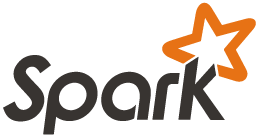
\includegraphics[width=0.4\linewidth]{spark-logo}
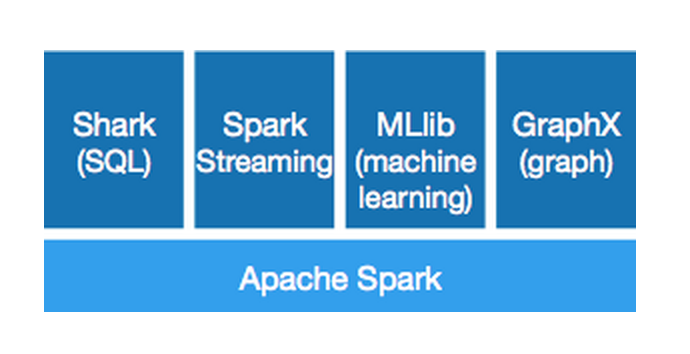
\includegraphics[width=\linewidth]{spark.png}
\caption{Spark powers a stack of high-level tools including Shark for SQL, MLlib for machine learning, GraphX, and Spark Streaming. These frameworks  cab be seamlessly combined in the same application.}
\end{marginfigure}

\begin{abstract}
We  argue for an early adoption of the rapidly maturing  Apache Spark\sidenote{\url{http://spark.apache.org/}} engine based ecosystem for  big data computations in astrophysics, especially in the light of the LSST project.  Spark provides a unified framework for a large gamut of data analysis requirements in astrophysics. We motivate the adoption of Spark in astrophysics by describing several use cases. 
\end{abstract}

\section{Types of Astrophysical Computations}
In the context of big data, there are three major types of Astrophysical computations: (a) \smallcaps{Query and aggregation}: frequent and fast query for astrophysical object over extensive databases, and summary statistics thereof; 
(b) \smallcaps{real time analysis:}  analysis of data as it streams from the telescope
(transients, supernovae, moving objects); (c) \smallcaps{analysis of archival data at scale:} classification, Fourier analysis, 
map-making, filtering, curve fitting, parameter estimation etc. on archival data. The standard in the astrophysical community has been applying different technologies for different problems: separate databases for queries, dedicated software stack for streaming analysis, and a slew of languages and platforms for archival data analysis.  This leads to frequent context switching for practitioners in the field, and makes it difficult to pursue projects that require live feedback between streaming analysis, querying and comparisons with archival data.  
\section{Where Spark Fits In}
Spark runs on top of Hadoop Distributed File System (HDFS) which is the de-facto industry standard for large scale data storage.  Spark enables querying databases via the Catalyst/Shark/BlinkDB SQL interface. The Spark Streaming tool enables real time analysis on streaming data (transients, supernovae, moving objects). Distributed machine learning  on archival  data sets (object detection, classification, photometric redshifts, supernova light curve fitting, etc.) can be performed using  MLLib,  a machine learning library built on top of Spark. Powerful statistical data exploration at scale can be performed with SparkR - a package for the R statistical language that enables R-users to leverage Spark functionality interactively from within the R shell. Relational (graph structured) data analysis can be performed using GraphX tool built on top of Spark.  Another great advantage of Spark is its Python API - pyspark -- that lets the end user develop applications in Python  -- a language that has already become extremely popular in  the astrophysics community. 



\section{Use Cases} 
\section{Future Directions}
\end{document}